% !TEX program = xelatex
\documentclass{article}
\usepackage[utf8]{inputenc}
\usepackage{amsmath}
\usepackage{relsize}
\usepackage{amssymb}
\usepackage{mathabx}
\usepackage{amsthm}
\usepackage{graphicx}
\usepackage[usenames,dvipsnames]{xcolor}
\newcommand{\kacper}[1]{ \bf  { \color{Orchid}{Kc: #1}}  }

\newtheorem{definition}{Definition}
\newtheorem{lemma}{Lemma}
\newtheorem{Theorem}{Theorem}
\newtheorem{example}{Example}
\newtheorem{statement}{Statement}
\newtheorem{corollary}{Corollary}
\newtheorem{test}{Test}
\newtheorem{proposition}{Proposition}

\newtheorem*{remark}{Remark}
\newenvironment{claim}[1]{\par\noindent\underline{Claim:}\space#1}{}
\newenvironment{claimproof}[1]{\par\noindent\underline{Proof:}\space#1}{\hfill $\blacksquare$}

\title{Testing MCMC convergence}
\author{}
\date{}



\begin{document}

\maketitle

Let $g(x,y)$ be a characteristic, analytic kernel. Let $p$ be a probability measure on $R^d$; suppose it has a density which logarithm exists, and is differentiable. Consider the following transform of $R^d$ valued random variable $X$
\begin{align}
 \mu_p(y) = E  \nabla \log p(X) g(X,y) - E \nabla g(X,y)
\end{align}
this transform is closely connected to Stein method and kernel mean embedding.

\section{test}
Let 
\begin{align}
 s(X,y) = \nabla \log p(X) g(X,y) -  \nabla g(X,y)
\end{align}
$J$ is number of frequencies.
\begin{equation}
 Z_i = ( s(X_i,Y_1) , \cdots, s(X_i,Y_J)  )\in \mathbf R^J.
\end{equation}

We define the vector of mean empirical differences 
$W_n = \frac 1  n \sum_{i=1}^n Z_i, $
and its covariance matrix
$\Sigma_n = \frac 1  n Z Z^{T}$.
The test statistic is
\begin{equation}
 S_n = n W_n \Sigma_n^{-1} W_n.
\end{equation}
The computation of $S_n$ requires inversion of a $J\times J$ matrix $\Sigma_n$, but this is fast and numerically stable: $J$ will typically be small, and is less than 10 in our experiments. The next proposition demonstrates the use of $S_n$ as a two-sample test statistic.
\begin{proposition}[Asymptotic behavior of $S_n$]
\label{prop:Hotelling}
 Let $d_{\mu,J}^2(P,Q)=0$ a.s. and let $\{X_i\}_{i=1}^n$ and $\{Y_i\}_{i=1}^n$  be i.i.d. samples from $P$ and $Q$ respectively. Then the statistic $S_n$ is a.s. asymptotically distributed as a $\chi^2$-random variable with $J$ degrees of freedom (as $n \to \infty$ with $d$ fixed). If $d_{\mu,J}^2(P,Q)>0$ a.s., then a.s. for any fixed $r$, $\mathbb P(S_n > r) \to 1$  as $n \to \infty$ .
\end{proposition}
We now apply the above proposition to obtain a statistical test. 

\begin{test}[MCMC convergence]
\label{test}
Calculate $S_n$. Choose a threshold $r_\alpha$ corresponding to the $1-\alpha$ quantile of a  $\chi^2$ distribution with $J$ degrees of freedom, and reject the null hypothesis whenever $S_n$ is larger than $r_\alpha$. 
\end{test}


\section{Math}

\begin{statement}
 If $X$ is distributed according to $p$ then the function  $\mu_p(y)$ is identically equal to zero  
\end{statement}
\begin{proof}
 For a fixed $y$ this is consequence of Stein method with as described in those guys NIPS paper. Or one can do integration by parts.   
\end{proof}

\begin{statement}
 If $X$ is not distributed according to $p$, but has a density, then $\mu_p(y)$ is different form zero almost everywhere. 
\end{statement}
\begin{proof}
THIS IS A SKETCH-- which means it's technically not a proof, but you may convince yourself it's true (if it is, but code seems to approve).
 Suppose $X$ is distributed according to density $p'$, then

\begin{align}
\mu_p(y) =& \int_{R^d} ( \nabla \log p(x) g(x,y) -  \nabla g(x,y)) p'(x) dx \\
          & \int_{R^d} g(x,y) \frac{ p'(x)}{p(x)} \nabla p(x) - \nabla g(x,y) p'(x)  
\end{align}
Integration by parts and shows that for all partial derivatives 
\begin{align}
0 = \int_{R} \frac{ \partial g(x,y)p'(x)} { \partial x_i } dx_i
\end{align}
\begin{align} 
 \int_{R} \frac{ \partial g(x,y) } { \partial x_i } p'(x) d x_i =
 -\int_{R} \frac{ \partial p(x) } { \partial x_i } g(x,y) d x_i 
\end{align}
So
\begin{align}
\mu_p(y) =& \int_{R^d} g(x,y) \frac{ p'(x)}{p(x)} \nabla p(x) -  g(x,y) \nabla p'(x)  \\
	 =& \int_{R^d} g(x,y) \left( \frac{ p'(x)}{p(x) } \nabla p(x) -  \nabla p'(x) \right)
\end{align}
 We would like to say that $t(x) = \frac{ p'(x)}{p(x) } \nabla p(x) -  \nabla p'(x)$  is kind of bounded and invoke the argument that $\mu_p$ is analytic, but first we need to prove that $t(x)$ is non-zero. 
 It is sufficient to see that $t(x) =0$ implies that $\nabla [ \log( p(x)) - \log( p'(x)) ]=0$, which implies that $p(x) = p'(x)e^C$. Since both $p$ and $p'$ are probability measures,  $C$ must be equal to 0.
 
 $\mu_p$ lives in the $RKHS$ associated with kernel $g$. Indeed if the integral exists 
 \[
  \int f(x) t(x) 
 \]
 then there exist an element $\mu_t$, such that $<\mu_t, f>$ is equal to above integral and in addition to that 
 \[
  \mu_t(t) = < \mu_t, k(t,\cdot)> = \int k(t,x) t(x) = \mu_p(t). 
 \]
The sufficient condition for $\int f(x) t(x)$ to exist is that 
\[
 \int <f, k(x,)> t(x) = < f, \int k(x,) t(x) > 
\]
$\int k(x,) t(x) $ exists and this one is easily verifiable for popular kernel (e.g. exists for exponential families and Gaussian kernel). By the lemma form our previous paper we see that $\mu_p(t)$ is  analytic. 
\end{proof}

\paragraph{Temporal dependence -- not an issue}
There are several ways to deal with temporal dependence, all of which, to our knowledge, work only asymptotically. Options include estimating auto-covariances, performing bootstrap or thinning. The last one, usually avoided in time-series analysis due to it's wasteful approach to data, is quite feasible in this application. It is also equally or less computationally complex then other options (potentially less noisy then estimating the auto covariance).      

It's obvious, but needs to show formally, that distribution of the test statistic under the null hypothesis, as $n$ approaches infinity, is as if we had used IID data. This is proved in appendix.

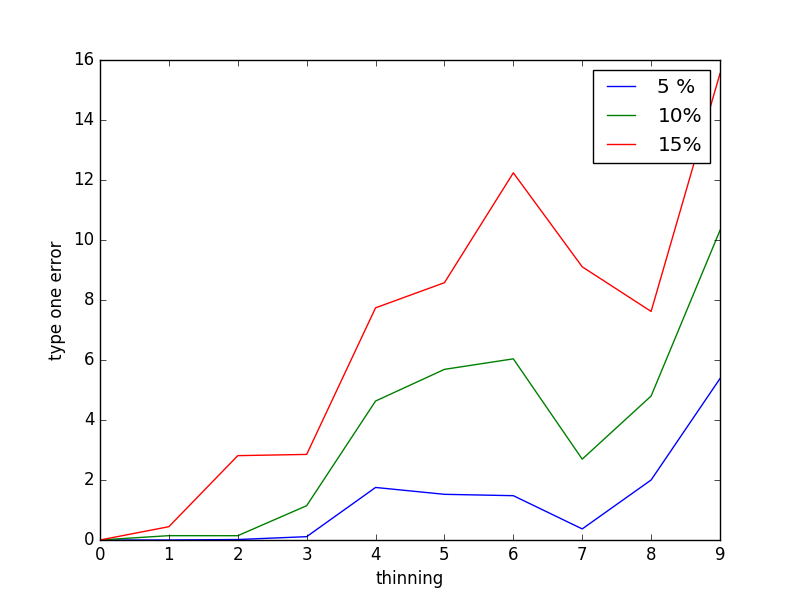
\includegraphics[width=0.8\textwidth]{type1.png}

\section{Sample selection}
So far we have not discussed problem problem of selecting sample from stationary distribution. In this section we propose a procedure that returns a sample for which it can not be rejected that it was generated from null distribution. We will proceed similarly to Heidelberger-Welch procedure, but is simpler way. We will generate blocks of samples and run test on them until we accept of world ends. 

\paragraph{type One-error}
We will use simple Bonferroni correction to deal with type one error. Tests level must be adjusted, so that they sum up to $\alpha$. Any scheme can be used, we use $\frac{1}{x^2}$ since we believe (am I turning  Bayesian?) that chains converge fast on average (faster than precision of the test that we are using).   

\paragraph{Type two}
Type two is somehow more complicated. In general (this is my intuition from finite state Markov chains and AR processes ) chain does not converge to stationary distribution in any number of finite steps, unless it has started for the stationary distribution. As usually in testing, one has no finite sample control over type two error. We can however infer what misspecified log probability would have given similar results on the given sample. This can be done by perturbing log probability in some direction and calculating the statistic on our sample. The magnitude of perturbation will show which models appear to be indistinguishable (now talk about parameters inference and that its even more difficult )    


\paragraph{Stupid fucked up SGLD}

\begin{equation}
 p(x, \theta) = C 0.5 \exp( -(x-\theta_1)^2/ 2\sigma_x^2 - ) + C 0.5 \exp( -(x-\theta_1 - \theta_2)^2/ 2\sigma_x^2)
\end{equation}















\end{document}


